\documentclass[a4paper,10pt]{article} 
\usepackage[utf8]{inputenc}
\usepackage[a4paper]{geometry}
\usepackage[magyar]{babel}
\usepackage{t1enc}
\usepackage{amsmath}
\usepackage{amssymb}
\usepackage{pgf,tikz,longtable}
\usetikzlibrary{arrows}
\frenchspacing 
\pagestyle{empty}
\newcommand{\ki}[2]{\hfill {\it #1 (#2)}\medskip}
\newcommand{\vonal}{\hbox to \hsize{\hskip2truecm\hrulefill\hskip2truecm}}
\newcommand{\degre}{\ensuremath{^\circ}}
\newcommand{\tg}{\mathop{\mathrm{tg}}\nolimits}
\newcommand{\ctg}{\mathop{\mathrm{ctg}}\nolimits}
\newcommand{\arc}{\mathop{\mathrm{arc}}\nolimits}
\begin{document}
\begin{center} \Large {\em 23. Nemzetközi Magyar Matematika Verseny} \end{center}
\begin{center} \large{\em Csíkszereda, 2014. március 12-16.} \end{center}
\smallskip
\begin{center} \large{\bf 11. osztály} \end{center}
\bigskip


{\bf 1. feladat: } Milyen szabály szerint írtuk le a $$2, 10, 16, 32, 42, 66, 80,
112, 130, 170$$ számokat? Ezt a szabályt folytatva, add meg a
    \[
        2, 10, 16, 32, 42, 66, 80, 112, 130, 170, \ldots
    \]
    sorozat általános tagjának a képletét!


\ki{dr. Kántor Sándorné}{Debrecen}\medskip



{\bf Megoldás: }  Írjuk fel az adott sorozat szomszédos tagjai különbségének a sorozatát,
 vagyis a differenciasorozatot: $$8, 6, 16, 10, 24, 14, 32, 18, 40,
 \ldots$$
 A differenciasorozat  páratlan sorszámú tagjai a  $8, 16, 24,
 \ldots$ számtani sorozat tagjai. A differenciasorozat  páros sorszámú tagjai
a $6, 10, 14, \ldots$ számtani sorozat tagjai. Az eredetileg adott
sorozat $n$-edik tagja $$a_n = 1\cdot 2 + 1\cdot8 + 3 \cdot2 +2
\cdot 8+ 5\cdot 2+ 3\cdot 8+ \ldots .$$ Ha $n$ páratlan, azaz  ha $n
= 2k + 1,$ alakú, akkor $$a_{2 k + 1} = 2 [( 1+ 3 + \ldots + (2 k
+1) ] + 8 ( 1 + 2 + 3 + \ldots + k)=$$
$$=2(k + 1)^2 + 8\frac{k^2+k}{2}=6k^2+8k+2=6\left(
\frac{n-1}{2}\right)^2+8\frac{n-1}{2}+2,$$ mivel $k=\frac{n-1}{2}.$
Így páratlan $n$-re \[{a_n} = \frac{3}{2}{n^2} + n -
\frac{1}{2}.\] Páros $n$-ekre, azaz $n = 2 k,$ esetén $$a_{2 k} =
2[1 + 3 +\ldots + (2 k-1)]+ 8 (1+ 2+\ldots + k).$$ Innen az 
előzőhöz hasonlóan kapjuk, hogy $$a_{2 k} = 2{k^2} + 8\frac{{{k^2}
+ k}}{2} = 6{k^2} + 4k.$$ Itt $n = 2 k$ miatt $k$ helyére $\frac
n2$-t írva, páros $n$-ekre $$a_n= \frac 32 n^2+2n.$$

\medskip

\textit{Megjegyzés}: Az $a_n$ képlet egységes formában is felírható,
figyelembe véve, hogy a páros és a páratlan sorszámú tagok közti
különbség $\frac{2n+1}{2}.$ Az általános tag tehát:
\[{a_n} = \frac{3}{2}{n^2} + \frac{3}{2}n - \frac{1}{4} + {\left( { - 1} \right)^n}\left( {\frac{{2n + 1}}{4}} \right).\]

\medskip

\vonal

{\bf 2. feladat: } Oldd meg az $\displaystyle x^{\log_3 64} = x^2\cdot8^{\log_3 x} -
x^{\log_3 8}$ egyenletet a valós számok halmazán!

\ki{Balázsi Borbála}{Beregszász}\medskip

{\bf Megoldás: }  Az egyenlet értelmezési tartománya a pozitív valós számok halmaza.
Mivel $a^{\log_b c}=c^{\log_b a}$, ha $a,b,c>0$ és $b\ne1$, az
egyenlet átírható
$$8^{\log_3 x}=x^2-1$$ alakba. Az $y={\log _3}x$ jelöléssel ${x^2}
= {9^y},$ tehát az egyenlet \[{8^y} = {9^y} - 1.\] Innen
\[{\left( {\frac{8}{9}} \right)^y} + {\left( {\frac{1}{9}}
\right)^y} = 1.\] A bal oldalon egy szigorúan csökkenő függvény
van, ezért az egyenletnek legfeljebb egy gyöke lehet. Ez a gyök $y =
1$, és így az eredeti egyenletnek $x = 3$ az egyetlen
megoldása.

\medskip

\vonal


{\bf 3. feladat: } Legfeljebb hány elemet tartalmazhat a $$H = \{1,2,3,\dots, 25\}$$
halmaznak az a részhalmaza, amelyben bármely két szám
 szorzata nem négyzetszám? Adj meg egy ilyen részhalmazt!


\ki{Bíró Béla}{Sepsiszentgyörgy}\medskip


{\bf Megoldás: }  Legyen $K$ a keresett részhalmaz. Mivel bármely két teljes négyzet szorzata is teljes négyzet,
 ezért a $K$-ban legfennebb egyetlen négyzetszám lehet. Vagyis az $1$,$4$,$9$,$16$, $25$ számok
 közül pontosan egy szerepelhet $K$-ban. Az általánosság leszűkítése nél\-kül feltételezhetjük,
 hogy $1\in K.$ Másrészt az $\{5,20\},$ $\{3,12\}$ illetve $\{6,24\}$ számpárok komponensei
közül legfennebb egy-egy szerepelhet $K$-ban, mert a párok
komponenseinek szorzata teljes négyzet. Harmadrészt a ${2,8,18}$
számhármasból legfennebb egy komponens szerepelhet $K$-ban, mert
közülük bármely kettőnek a szorzata teljes négyzet. Innen
következik, hogy a $K$-ban legfennebb $25-4-3-2 = 16$ szám
szerepelhet. Negyedrészt bizonyítható, hogy ez a $16$-os elemszám
elérhető. Például a
$$K =\{1,2,3,5,6,7,10,11,13,14,15,17,19,21,22,23\}$$ részhalmaz
teljesíti a feladat feltételeit.

\medskip

\vonal

{\bf 4. feladat: } Az $e$ és $f$ egyenesek párhuzamosak és egymástól
egységnyi távolságra vannak. Vedd fel az $e$ egyenesen az
$A_1,$ $A_2,$ $A_3,$ $\dots, A_n, A_{n+1}$ pontokat és az $f$
egyenesen a $B_1, B_2, \dots, B_n,$ $B_{n+1}$ pontokat úgy, hogy
mindkét egyenesen bármely két szomszédos pont távolsága
egységnyi, és minden $i\in\mathbb{N}$, $1\le i\le n+1$ számra
az $A_iB_i$ szakasz merőleges az $e$ és $f$ egyenesekre. Kösd
össze az $A_1$ pontot a $B_n$ és $B_{n+1}$ pontokkal. Az
összekötő sza\-ka\-szok az $A_2B_2$ szakaszt rendre a $P$
és $Q$ pontokban metszik.

a) Van-e olyan pozitív egész $n$ szám, amelyre az $A_1PQ$
háromszög területe $\displaystyle \frac{1}{1802}$
területegység?

b) Van-e olyan pozitív egész $n$ szám, amelyre az $A_1PQ$
háromszög területe $\displaystyle \frac{1}{1860}$
területegység?

\ki{Bíró Bálint}{Eger}\medskip

{\bf Megoldás: } a) A szöveg alapján $A_iA_{i+1}B_{i+1}B_i$ egységnyi oldalú
négy\-ze\-tek, amelyek a következő vázlatos ábrának megfelelően he\-lyez\-ked\-nek el.

\begin{center}
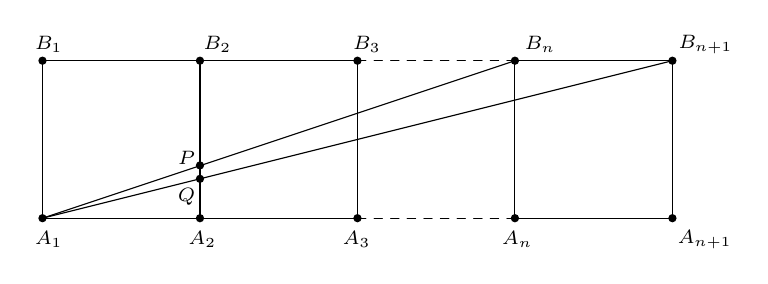
\begin{tikzpicture}[line cap=round,line join=round,>=triangle 45,x=1.0cm,y=1.0cm]
\draw (0,2)-- (2,2); \draw (2,2)-- (4,2); \draw [dash pattern=on 3pt
off 3pt] (4,2)-- (6,2); \draw (6,2)-- (8,2); \draw (0,4)-- (2,4);
\draw (2,4)-- (4,4); \draw [dash pattern=on 3pt off 3pt] (4,4)--
(6,4); \draw (6,4)-- (8,4); \draw (2,4)-- (2,2); \draw (0,2)--
(0,4); \draw (4,4)-- (4,2); \draw (6,4)-- (6,2); \draw (8,4)--
(8,2); \draw (0,2)-- (8,4); \draw (0,2)-- (6,4);
\begin{scriptsize}
\fill [color=black] (0,2) circle (1.5pt); \draw[color=black]
(0.08,1.73) node {$A_1$}; \fill [color=black] (2,2) circle (1.5pt);
\draw[color=black] (2.03,1.73) node {$A_2$}; \fill [color=black]
(4,2) circle (1.5pt); \draw[color=black] (3.99,1.73) node {$A_3$};
\fill [color=black] (6,2) circle (1.5pt); \draw[color=black]
(6.03,1.73) node {$A_n$}; \fill [color=black] (8,2) circle (1.5pt);
\draw[color=black] (8.41,1.73) node {$A_{n+1}$}; \fill [color=black]
(0,4) circle (1.5pt); \draw[color=black] (0.08,4.21) node {$B_1$};
\fill [color=black] (2,4) circle (1.5pt); \draw[color=black]
(2.22,4.21) node {$B_2$}; \fill [color=black] (4,4) circle (1.5pt);
\draw[color=black] (4.12,4.21) node {$B_3$}; \fill [color=black]
(6,4) circle (1.5pt); \draw[color=black] (6.32,4.21) node {$B_n$};
\fill [color=black] (8,4) circle (1.5pt); \draw[color=black]
(8.42,4.21) node {$B_{n+1}$}; \fill [color=black] (2,2.67) circle
(1.5pt); \draw[color=black] (1.83,2.77) node {$P$}; \fill
[color=black] (2,2.5) circle (1.5pt); \draw[color=black] (1.83,2.27)
node {$Q$};
\end{scriptsize}
\end{tikzpicture}
\end{center}

A megfelelő szögek egyenlősége miatt az $A_1A_2P$ és
${A_1}{A_n}{B_n}$ háromszögek hasonlók, ezért megfelelő oldalaik
aránya egyenlő, azaz $\frac{A_1A_2}{PA_2}=\frac{A_1A_n}{A_nB_n}.$
Ebből $A_1A_2=A_nB_n=1$ és $A_1A_n=n-1$ miatt $P{A_2} =
\frac{1}{{n - 1}}.$ Nyilvánvaló, hogy $n \ne 1$, hiszen ha csak egy
négyzet szerepelne az ábrán, akkor a $P,Q$ pontok nem jöhetnének
létre. A megfelelő szögek egyenlősége miatt az ${A_1}{A_2}Q$
és $A_1A_{n+1}B_{n+1}$ háromszögek szintén hasonlók, ezért
megfelelő olda\-la\-ik aránya egyenlő, vagyis
$$\frac{{{A_1}{A_2}}}{{Q{A_2}}} = \frac{{{A_1}{A_{n + 1}}}}{{{A_{n +
1}}{B_{n + 1}}}}.$$ Ez alapján $Q{A_2} = \frac{1}{n},$ tehát
$$PQ = P{A_2} - Q{A_2} = \frac{1}{{n - 1}} - \frac{1}{n} =
\frac{1}{{n \cdot \left( {n - 1} \right)}}.$$ Az ${A_1}PQ$
háromszögnek a $PQ$ oldalhoz tartozó magassága az ${A_1}{A_2} = 1$
szakasz, ezért a háromszög   területére azt kapjuk, hogy
 $$T = \frac{{PQ \cdot {A_1}{A_2}}}{2} = \frac{1}{{2n \cdot \left(
{n - 1} \right)}}.$$ Ha az $A_1PQ$ háromszög területe $\displaystyle
\frac{1}{1802},$ akkor $$2n \cdot \left( {n - 1} \right) = 1802.$$
Ennek az egyenletnek nincs pozitív egész megoldása, mert 
$n \cdot \left( {n - 1} \right)$ páros szám, így a bal oldala
$4$-gyel osztható, míg $1802$ nem osztható $4$-gyel, tehát az a)
kérdésre a válasz az, hogy ilyen $n$ nem létezik.

Ha az ${A_1}PQ$ háromszög területe $\frac{1}{{1860}}$, akkor
$\frac{1}{{2n \cdot \left( {n - 1} \right)}} = \frac{1}{{1860}}$,
vagyis $2n \cdot \left( {n - 1} \right) = 1860$, ahonnan
 ${n^2} - n - 930 = 0.$
 
\newpage 
A megoldások ${n_1} = 31$ és ${n_2} =  - 30.$ Az ${n_2} =  - 30$
nyilván nem felel meg a feltételeknek, tehát a b) kérdésre $n =
31$ a válasz.

\medskip

\vonal

{\bf 5. feladat: } Egy szabályos kilencszögben meghúztuk az összes átlót.
 Van-e a kilencszög belsejében olyan pont, amelyre legalább három átló
 illeszkedik?

\ki{Zsombori Gabriella}{Csíkszereda}

\ki{dr. András Szilárd}{Kolozsvár}\medskip

{\bf Megoldás: } A szabályos kilencszög szögei
$140^{\circ}$-osak. (Egy sza\-bályos $n$-oldalú sokszög
szögeinek összege $(n-2)\cdot180^{\circ}$, tehát egyik
szöge $\frac{(n-2)\cdot180^{\circ}}{n}$.) Ekkor egy oldalt
közrefogó kerületi szög mértéke
$\alpha=20^{\circ}$. Tételezzük fel, hogy van három
olyan átló, amelyek a kilencszög belsejében
összefutnak. Ekkor ezek közül semelyik kettő nem
találkozhat ugyanabban a csúcsban. A mellékelt
ábrán vastagítva látható ez a három
átló. Ugyanakkor az ábrán két csúcs
közé beírt $k_{i}$ nullától
különböző természetes szám jelentse azt,
hogy az $\alpha=20^{\circ}$ hányszorosát fogja közre
ehhez a két csúcshoz tartozó kerületi szög
($i\in\left\{  1,2,3,4,5,6\right\}  $).
\begin{center}
\includegraphics[width=0.5\textwidth]{ceva1.eps}%
\end{center}
Ekkor
\[
k_{1}+k_{2}+k_{3}+k_{4}+k_{5}+k_{6}=9
\]
és a Ceva-tétel trigonometrikus alakját felírva:
\[
\frac{\sin\left(  k_{1}\alpha\right)  }{\sin\left(  k_{2}\alpha\right)  }%
\cdot\frac{\sin\left(  k_{3}\alpha\right)  }{\sin\left(
k_{4}\alpha\right) }\cdot\frac{\sin\left(  k_{5}\alpha\right)
}{\sin\left(  k_{6}\alpha\right) }=1.
\]
 A $k_{1},k_{2},k_{3},k_{4},k_{5},k_{6}$ nullától
különböző természetes számokat rendezzük
növekvő sorrendbe. Ekkor az első nem lehet $1$-nél
na\-gyobb (ha legalább $2$ lenne, akkor a hat szám
összege legalább $12$ lenne). Hasonló
meggondolásból a második és a harmadik
szám sem lehet $1$-nél nagyobb. Ekkor $k_{1},k_{2},k_{3},k_{4}%
,k_{5},k_{6}$ lehetséges - növekvő sorrendbe szedett -
értékei:%
$$\left\{  1,1,1,1,1,4\right\}  \quad \left\{  1,1,1,1,2,3\right\}
\quad \left\{  1,1,1,2,2,2\right\}  $$%

$\bullet$ $\left\{  1,1,1,1,1,4\right\}  $ esetén a
trigonometrikus
összefüggés%
\[
\frac{\sin\alpha}{\sin\alpha}\cdot\frac{\sin\alpha}{\sin\alpha}\cdot\frac
{\sin4\alpha}{\sin\alpha}=1\mbox{ vagy }\frac{\sin\alpha}{\sin\alpha}%
\cdot\frac{\sin\alpha}{\sin\alpha}\cdot\frac{\sin\alpha}{\sin4\alpha}=1
\]
lenne és mindkettő a $\sin80^{\circ}=\sin20^\circ$
egyenlőséget eredményezné, ami nem igaz.

$\bullet$ $\left\{  1,1,1,1,2,3\right\}  $ esetén a
trigonometrikus összefüggésből 
$\sin40^{\circ}$ $=$ $\sin60^{\circ}$ vagy
$\sin40^{\circ}\sin60^{\circ}=\sin20^{\circ}\sin20^{\circ}$
következne, ami szintén lehetetlen. (A szinusz
függvény $0^{\circ} $ és $90^{\circ}$ között
szi\-go\-rúan növekvő és pozitív
értékeket vesz fel.)

$\bullet$ $\left\{  1,1,1,2,2,2\right\}  $ esetén szintén a
trigonometrikus összefüggésből $\left(
\sin20^{\circ}\right) ^{3}$ $=$ $\left(  \sin40^{\circ}\right) ^{3}$
vagy $\sin20^{\circ}$ $=$ $\sin40^{\circ}$ következne, ami nem
igaz. \newline Tehát nincs három olyan átló, amelyek
a kilencszög belsejében összefutnak.


{\bf 2. megoldás}: A mellékelt ábrán megfigyelhető, hogy három
típusú átlója van egy szabályos
kilencszögnek.

\begin{center}
\includegraphics[width=0.5\textwidth]{9szog.eps}%
\end{center}
Nevezzük $1$-es típusúnak azokat az átlókat (az
ábrán a vastagított szakaszok), amelyeknek egyik
oldalán pontosan egy csúcs\-pont található. Legyenek
$2$-es típusúak azok az átlók (az ábrán a
szaggatott szakaszok), amelyeknek egyik oldalán pontosan két
csúcspont található és $3$-as típusúak azok
az átlók, amelyeknek egyik oldalán pontosan három
csúcspont van.

Mivel az $1$-es típusú átlók egyik oldalán
pontosan egy csúcs\-pont van, ebből a csúcspontból
kell egy másik (ezt metsző) átló kiinduljon. Viszont
így nem marad csúcspont, amiből egy harmadik is
kiinduljon és az első kettővel összefusson.
Tehát az $\left\{  1,1\right\}  $, $\left\{  1,2\right\} $,
illetve $\left\{  1,3\right\}  $ metszéspontok nem lehetnek
összefutási pontok.

 Vizsgáljuk most a $\left\{
2,2\right\}  $ metszéspontokat. Ezek a metszéspontok mind
rajta vannak a kilencszög egy-egy olyan
szimmetria\-ten\-ge\-lyén, amelyek áthaladnak egy
csúcson. Ha a $\left\{ 2,2\right\} $ metszéspont az
ábrán látható típusú, akkor ez nem lehet
összefutási pont.
\begin{center}
\includegraphics[width=0.5\textwidth]{9szog_2atlo.eps}
\end{center}
Valóban, ha kiválasztunk egy csúcsot és ezen a
csúcson keresz\-tül behúzzuk a kilencszögnek a
szimmetriatengelyét, akkor az ehhez a csúcshoz
legközelebb eső csúcsok által meghatározott
$2$-es típusú átlók ezen szimmetriatengelyen
való metszéspontjáról van szó, így ez nem
lehet összefutási pont. \newline Ebből következik,
hogy a $\left\{  2,2\right\}  $ másik típusú
metszéspontok sem lehetnek összefutási pontok (nem
eshetnek egybe az első típusú $\left\{  2,2\right\}  $
metszéspontokkal és szimmetriatengelyen vannak - lásd az
ábrát). Hasonlóan tárgyalható le az is, hogy a
$\left\{ 3,3\right\}  $ metszéspontok sem lehetnek
összefutási pontok. Hátra van még a $\left\{
2,3\right\}  $ metszéspontok vizsgálata. Ezek a
metszéspontok eddigi egyetlen metszésponttal sem eshetnek
egybe. Ezen kívül, ha megfigyeljük a mellékelt
ábrát, egy kiválasztott csúcsból húzott, $a$
szim\-met\-riatengelyen találkozó $2$-es típusú
átlók (azok, amelyeknek a talál\-kozási pontja a
csúcshoz a lehető leg\-kö\-ze\-lebb esik, de nem esik
egybe azzal) ugyanabból a csúcsból induló $3$-as
típusú átlókkal négy különböző
metszéspontot határoznak meg. Tükrözzük ezt a
négy metszéspontot a $b$ szimmetriatengelyre nézve, az
ábrán látható módon. Ekkor négy újabb
$\left\{  2,3\right\}  $ metszéspontot kapunk.
\begin{center}
\includegraphics[width=0.45\textwidth]{9szog_2atlo_2.eps}\hfill
\includegraphics[width=0.45\textwidth]{9szog_23atlo.eps}%
\end{center}
A két-két - $b$ tengelyhez közelebb eső -
metszéspont egyike sem eshet a $b$ tengelyre (ezáltal
egybeesve egy másikkal), mivel ezen pontok $b$ tengelyen
találkozó tartóegyenesei azonos típusúak (ezek
pedig nem lehetnek összefutási pontok).\newline Tehát
nincs három olyan átló, amelyek összefutnának.



\textit{Megjegyzés}: P. L. Wantzel bizonyította be $1837$-ben, hogy ha az $n$
természetes szám páratlan prímtényezői nem
különböző Fermat-prímek, akkor a szabályos
$n$-szög nem szer\-keszt\-he\-tő meg körzővel és
vonalzóval. Mivel a $9$ prímtényezői nem
különbözőek, ezért a szabályos
kilencszög nem szerkeszthető meg euklideszi
eszközökkel. (Fermat-prímeknek az $F_{n}=2^{2^{n}}+1$
alakú prímszámokat nevezzük, ahol $n$
természetes szám. A jelenleg ismert Fermat-prímek:
$F_{0}=3$, $F_{1}=5$, $F_{2}=17$, $F_{3}=257,$ és 
$F_{4}=65537.$)


\medskip

\vonal

{\bf 6. feladat: } a) Határozd meg a síknak egy\-ségoldalú szabályos
háromszögekkel, egy\-ség\-oldalú négyzetekkel és
egységoldalú sza\-bályos hatszögekkel való összes
szabályos le\-fö\-dé\-sét! Egy lefödés azt jelenti, hogy
a sokszögek hézag és átfödés nélkül (egyrétűen)
lefödik a síkot. A lefödés szabályos, ha léteznek olyan
$a,b$ és $c$ nullától különböző természetes
számok, amelyekre minden keletkező csúcs körül pontosan
$a$ darab háromszög, $b$ darab négyzet és $c$ darab
hatszög van, valamilyen rögzített sorrendben.

b) Bizonyítsd be, hogy létezik végtelen sok olyan, nem
fel\-tétle\-nül szabályos lefödés, a\-mely\-hez
hozzárendelhető valamilyen $a,b$ és $c$ nullától
különböző természetes szám úgy, hogy minden
keletkező csúcs körül pontosan $a$ darab háromszög, $b$
darab négyzet és $c$ darab hatszög legyen!

\ki{Zsombori Gabriella}{Csíkszereda}

\ki{dr. András Szilárd, dr. Lukács Andor}{Kolozsvár}\medskip

{\bf Megoldás: } Javasoljuk elolvasni mind a négy évfolyam utolsó feladatának
a megoldását az évfolyamok sorszámának nö\-vek\-vő
sorrendjében. Az a) pont megoldásához észrevesszük,  hogy
egy csúcs\-pontban négy vagy öt alakzat találkozhat.

Abban az esetben, ha csak négy alakzat találkozik, a
következő eseteket különböztetjük meg:

$\bullet$ Ha ezek között egy hatszög, $a$ darab háromszög
és $b$ darab négyzet, akkor
        \[
            a\cdot 60^\circ + b\cdot 90^\circ + 120^\circ = 360^\circ.
        \]
        Így a $\left\{ \begin{array}{rl}
            2a + 3b &= 8 \\ a + b &= 3
        \end{array}\right.$ egyenletrendszert kell megoldanunk a po\-zi\-tív egész számok halmazán, aminek a megoldása $a=1$ és $b=2$. Tehát csak a $(3,4,4,6)$ és $(4,3,4,6)$ elrendezések lehetségesek egy csúcs körül:
        \begin{center}
        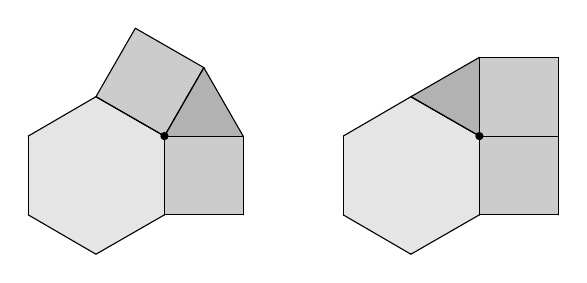
\begin{tikzpicture}[line cap=round,line join=round,>=triangle 45,x=1.0cm,y=1.0cm]

\fill[fill=black,fill opacity=0.1] (2,1) -- (2,2) -- (1.13,2.5) -- (0.27,2) -- (0.27,1) -- (1.13,0.5) -- cycle;
\fill[fill=black,fill opacity=0.2] (2,2) -- (2,1) -- (3,1) -- (3,2) -- cycle;
\fill[fill=black,fill opacity=0.2] (1.13,2.5) -- (2,2) -- (2.5,2.87) -- (1.63,3.37) -- cycle;
\fill[fill=black,fill opacity=0.3] (2,2) -- (3,2) -- (2.5,2.87) -- cycle;
\fill[fill=black,fill opacity=0.1] (6,1) -- (6,2) -- (5.13,2.5) -- (4.27,2) -- (4.27,1) -- (5.13,0.5) -- cycle;
\fill[fill=black,fill opacity=0.2] (6,2) -- (6,1) -- (7,1) -- (7,2) -- cycle;
\fill[fill=black,fill opacity=0.2] (6,2) -- (7,2) -- (7,3) -- (6,3) -- cycle;
\fill[fill=black,fill opacity=0.3] (6,3) -- (5.13,2.5) -- (6,2) -- cycle;
\draw (2,1)-- (2,2);\draw (2,1)-- (2,2);
\draw (2,2)-- (1.13,2.5);
\draw (1.13,2.5)-- (0.27,2);
\draw (0.27,2)-- (0.27,1);
\draw (0.27,1)-- (1.13,0.5);
\draw (1.13,0.5)-- (2,1);
\draw (2,2)-- (2,1);
\draw (2,1)-- (3,1);
\draw (3,1)-- (3,2);
\draw (3,2)-- (2,2);
\draw (1.13,2.5)-- (2,2);
\draw (2,2)-- (2.5,2.87);
\draw (2.5,2.87)-- (1.63,3.37);
\draw (1.63,3.37)-- (1.13,2.5);
\draw (2,2)-- (3,2);
\draw (3,2)-- (2.5,2.87);
\draw (2.5,2.87)-- (2,2);
\draw (6,1)-- (6,2);
\draw (6,2)-- (5.13,2.5);
\draw (5.13,2.5)-- (4.27,2);
\draw (4.27,2)-- (4.27,1);
\draw (4.27,1)-- (5.13,0.5);
\draw (5.13,0.5)-- (6,1);
\draw (6,2)-- (6,1);
\draw (6,1)-- (7,1);
\draw (7,1)-- (7,2);
\draw (7,2)-- (6,2);
\draw (6,2)-- (7,2);
\draw (7,2)-- (7,3);
\draw (7,3)-- (6,3);
\draw (6,3)-- (6,2);
\draw (6,3)-- (5.13,2.5);
\draw (5.13,2.5)-- (6,2);
\draw (6,2)-- (6,3);
\begin{scriptsize}
\fill [color=black] (2,2) circle (1.5pt);
\fill [color=black] (6,2) circle (1.5pt);
\end{scriptsize}
\end{tikzpicture}
\end{center}

Ha két hatszög van, akkor az előbbi jelöléseket alkalmazva
\[
    a\cdot 60^\circ + b\cdot 90^\circ + 240^\circ = 360^\circ
\]
összefüggés kell teljesüljön. Mivel ebben az esetben $a+b = 2$ is fennáll,
 nincs megoldásunk.

$\bullet$ Abban az esetben, ha egy csúcspontban öt alakzat
találkozik, mivel az alakzatok között kell legyen
háromszög, négyzet és hatszög is, a fennmaradt két
alakzat szögeinek összege $$360^\circ - (60^\circ + 90^\circ +
120^\circ) = 90^\circ$$ és ez nem lehetséges.

Tehát egy csúcspontban csak négy alakzat találkozhat. A $(4,3,4,6)$ elrendezés esetén lehet szabályos
lefödést szerkeszteni, és ez a lefödés egyértelmű.
Valóban, kiindulva a hatszög egyik $(4,3,4,6)$ típusú
csúcsából, ez a hatszög minden további csúcsát
egyértelműen meghatározza (mind $(4,3,4,6)$ típusúak
lesznek). De így a kialakult tizenkétszög csúcsai is
egyértelműen meghatározottak:
    \begin{center}
    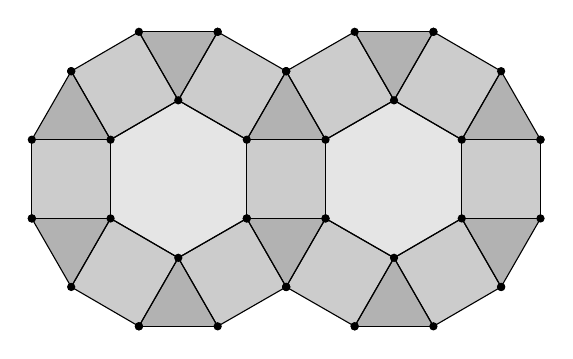
\begin{tikzpicture}[line cap=round,line join=round,>=triangle 45,x=1.0cm,y=1.0cm]
\fill[fill=black,fill opacity=0.1] (3,1) -- (3,2) -- (2.13,2.5) -- (1.27,2) -- (1.27,1) -- (2.13,0.5) -- cycle;
\fill[fill=black,fill opacity=0.1] (4,2) -- (4,1) -- (4.87,0.5) -- (5.73,1) -- (5.73,2) -- (4.87,2.5) -- cycle;
\fill[fill=black,fill opacity=0.2] (4,2) -- (3,2) -- (3,1) -- (4,1) -- cycle;
\fill[fill=black,fill opacity=0.3] (4,1) -- (3,1) -- (3.5,0.13) -- cycle;
\fill[fill=black,fill opacity=0.2] (4,2) -- (4.87,2.5) -- (4.37,3.37) -- (3.5,2.87) -- cycle;
\fill[fill=black,fill opacity=0.2] (4.87,2.5) -- (5.73,2) -- (6.23,2.87) -- (5.37,3.37) -- cycle;
\fill[fill=black,fill opacity=0.2] (5.73,2) -- (5.73,1) -- (6.73,1) -- (6.73,2) -- cycle;
\fill[fill=black,fill opacity=0.2] (5.73,1) -- (4.87,0.5) -- (5.37,-0.37) -- (6.23,0.13) -- cycle;
\fill[fill=black,fill opacity=0.2] (4.87,0.5) -- (4,1) -- (3.5,0.13) -- (4.37,-0.37) -- cycle;
\fill[fill=black,fill opacity=0.2] (3,1) -- (2.13,0.5) -- (2.63,-0.37) -- (3.5,0.13) -- cycle;
\fill[fill=black,fill opacity=0.2] (2.13,0.5) -- (1.27,1) -- (0.77,0.13) -- (1.63,-0.37) -- cycle;
\fill[fill=black,fill opacity=0.2] (1.27,1) -- (1.27,2) -- (0.27,2) -- (0.27,1) -- cycle;
\fill[fill=black,fill opacity=0.2] (1.27,2) -- (2.13,2.5) -- (1.63,3.37) -- (0.77,2.87) -- cycle;
\fill[fill=black,fill opacity=0.2] (2.13,2.5) -- (3,2) -- (3.5,2.87) -- (2.63,3.37) -- cycle;
\fill[fill=black,fill opacity=0.3] (3,2) -- (4,2) -- (3.5,2.87) -- cycle;
\fill[fill=black,fill opacity=0.3] (4.37,3.37) -- (4.87,2.5) -- (5.37,3.37) -- cycle;
\fill[fill=black,fill opacity=0.3] (6.23,2.87) -- (5.73,2) -- (6.73,2) -- cycle;
\fill[fill=black,fill opacity=0.3] (6.73,1) -- (5.73,1) -- (6.23,0.13) -- cycle;
\fill[fill=black,fill opacity=0.3] (5.37,-0.37) -- (4.87,0.5) -- (4.37,-0.37) -- cycle;
\fill[fill=black,fill opacity=0.3] (2.63,-0.37) -- (2.13,0.5) -- (1.63,-0.37) -- cycle;
\fill[fill=black,fill opacity=0.3] (0.77,0.13) -- (1.27,1) -- (0.27,1) -- cycle;
\fill[fill=black,fill opacity=0.3] (0.27,2) -- (1.27,2) -- (0.77,2.87) -- cycle;
\fill[fill=black,fill opacity=0.3] (1.63,3.37) -- (2.13,2.5) -- (2.63,3.37) -- cycle;
\draw (3,1)-- (3,2);
\draw (3,2)-- (2.13,2.5);
\draw (2.13,2.5)-- (1.27,2);
\draw (1.27,2)-- (1.27,1);
\draw (1.27,1)-- (2.13,0.5);
\draw (2.13,0.5)-- (3,1);
\draw (4,2)-- (4,1);
\draw (4,1)-- (4.87,0.5);
\draw (4.87,0.5)-- (5.73,1);
\draw (5.73,1)-- (5.73,2);
\draw (5.73,2)-- (4.87,2.5);
\draw (4.87,2.5)-- (4,2);
\draw (4,2)-- (3,2);
\draw (3,2)-- (3,1);
\draw (3,1)-- (4,1);
\draw (4,1)-- (4,2);
\draw (4,1)-- (3,1);
\draw (3,1)-- (3.5,0.13);
\draw (3.5,0.13)-- (4,1);
\draw (4,2)-- (4.87,2.5);
\draw (4.87,2.5)-- (4.37,3.37);
\draw (4.37,3.37)-- (3.5,2.87);
\draw (3.5,2.87)-- (4,2);
\draw (4.87,2.5)-- (5.73,2);
\draw (5.73,2)-- (6.23,2.87);
\draw (6.23,2.87)-- (5.37,3.37);
\draw (5.37,3.37)-- (4.87,2.5);
\draw (5.73,2)-- (5.73,1);
\draw (5.73,1)-- (6.73,1);
\draw (6.73,1)-- (6.73,2);
\draw (6.73,2)-- (5.73,2);
\draw (5.73,1)-- (4.87,0.5);
\draw (4.87,0.5)-- (5.37,-0.37);
\draw (5.37,-0.37)-- (6.23,0.13);
\draw (6.23,0.13)-- (5.73,1);
\draw (4.87,0.5)-- (4,1);
\draw (4,1)-- (3.5,0.13);
\draw (3.5,0.13)-- (4.37,-0.37);
\draw (4.37,-0.37)-- (4.87,0.5);
\draw (3,1)-- (2.13,0.5);
\draw (2.13,0.5)-- (2.63,-0.37);
\draw (2.63,-0.37)-- (3.5,0.13);
\draw (3.5,0.13)-- (3,1);
\draw (2.13,0.5)-- (1.27,1);
\draw (1.27,1)-- (0.77,0.13);
\draw (0.77,0.13)-- (1.63,-0.37);
\draw (1.63,-0.37)-- (2.13,0.5);
\draw (1.27,1)-- (1.27,2);
\draw (1.27,2)-- (0.27,2);
\draw (0.27,2)-- (0.27,1);
\draw (0.27,1)-- (1.27,1);
\draw (1.27,2)-- (2.13,2.5);
\draw (2.13,2.5)-- (1.63,3.37);
\draw (1.63,3.37)-- (0.77,2.87);
\draw (0.77,2.87)-- (1.27,2);
\draw (2.13,2.5)-- (3,2);
\draw (3,2)-- (3.5,2.87);
\draw (3.5,2.87)-- (2.63,3.37);
\draw (2.63,3.37)-- (2.13,2.5);
\draw (3,2)-- (4,2);
\draw (4,2)-- (3.5,2.87);
\draw (3.5,2.87)-- (3,2);
\draw (4.37,3.37)-- (4.87,2.5);
\draw (4.87,2.5)-- (5.37,3.37);
\draw (5.37,3.37)-- (4.37,3.37);
\draw (6.23,2.87)-- (5.73,2);
\draw (5.73,2)-- (6.73,2);
\draw (6.73,2)-- (6.23,2.87);
\draw (6.73,1)-- (5.73,1);
\draw (5.73,1)-- (6.23,0.13);
\draw (6.23,0.13)-- (6.73,1);
\draw (5.37,-0.37)-- (4.87,0.5);
\draw (4.87,0.5)-- (4.37,-0.37);
\draw (4.37,-0.37)-- (5.37,-0.37);
\draw (2.63,-0.37)-- (2.13,0.5);
\draw (2.13,0.5)-- (1.63,-0.37);
\draw (1.63,-0.37)-- (2.63,-0.37);
\draw (0.77,0.13)-- (1.27,1);
\draw (1.27,1)-- (0.27,1);
\draw (0.27,1)-- (0.77,0.13);
\draw (0.27,2)-- (1.27,2);
\draw (1.27,2)-- (0.77,2.87);
\draw (0.77,2.87)-- (0.27,2);
\draw (1.63,3.37)-- (2.13,2.5);
\draw (2.13,2.5)-- (2.63,3.37);
\draw (2.63,3.37)-- (1.63,3.37);
\begin{scriptsize}
\fill [color=black] (3,1) circle (1.5pt);
\fill [color=black] (3,2) circle (1.5pt);
\fill [color=black] (2.13,2.5) circle (1.5pt);
\fill [color=black] (1.27,2) circle (1.5pt);
\fill [color=black] (1.27,1) circle (1.5pt);
\fill [color=black] (2.13,0.5) circle (1.5pt);
\fill [color=black] (4,2) circle (1.5pt);
\fill [color=black] (4,1) circle (1.5pt);
\fill [color=black] (4.87,0.5) circle (1.5pt);
\fill [color=black] (5.73,1) circle (1.5pt);
\fill [color=black] (5.73,2) circle (1.5pt);
\fill [color=black] (4.87,2.5) circle (1.5pt);
\fill [color=black] (3,1) circle (1.5pt);
\fill [color=black] (4,1) circle (1.5pt);
\fill [color=black] (3.5,0.13) circle (1.5pt);
\fill [color=black] (4.37,3.37) circle (1.5pt);
\fill [color=black] (3.5,2.87) circle (1.5pt);
\fill [color=black] (6.23,2.87) circle (1.5pt);
\fill [color=black] (5.37,3.37) circle (1.5pt);
\fill [color=black] (6.73,1) circle (1.5pt);
\fill [color=black] (6.73,2) circle (1.5pt);
\fill [color=black] (5.37,-0.37) circle (1.5pt);
\fill [color=black] (6.23,0.13) circle (1.5pt);
\fill [color=black] (3.5,0.13) circle (1.5pt);
\fill [color=black] (4.37,-0.37) circle (1.5pt);
\fill [color=black] (2.63,-0.37) circle (1.5pt);
\fill [color=black] (3.5,0.13) circle (1.5pt);
\fill [color=black] (0.77,0.13) circle (1.5pt);
\fill [color=black] (1.63,-0.37) circle (1.5pt);
\fill [color=black] (0.27,2) circle (1.5pt);
\fill [color=black] (0.27,1) circle (1.5pt);
\fill [color=black] (1.63,3.37) circle (1.5pt);
\fill [color=black] (0.77,2.87) circle (1.5pt);
\fill [color=black] (3.5,2.87) circle (1.5pt);
\fill [color=black] (2.63,3.37) circle (1.5pt);
\fill [color=black] (3.5,2.87) circle (1.5pt);
\fill [color=black] (5.37,3.37) circle (1.5pt);
\fill [color=black] (6.73,2) circle (1.5pt);
\fill [color=black] (6.23,0.13) circle (1.5pt);
\fill [color=black] (4.37,-0.37) circle (1.5pt);
\fill [color=black] (1.63,-0.37) circle (1.5pt);
\fill [color=black] (0.27,1) circle (1.5pt);
\fill [color=black] (0.77,2.87) circle (1.5pt);
\fill [color=black] (2.63,3.37) circle (1.5pt);
\end{scriptsize}
\end{tikzpicture}
    \end{center}
Ha a $(3,4,4,6)$ csúcs körüli elrendezésből indulunk ki
és egy hatszög csúcsait körbejárjuk, szükségszerűen
az összes többi csúcs is $(3,4,4,6)$ típusú lesz. Viszont
így a  felhasznált háromszögek harmadik csúcsai
$(4,3,4,6)$ típusúak lesznek:
    \begin{center}
    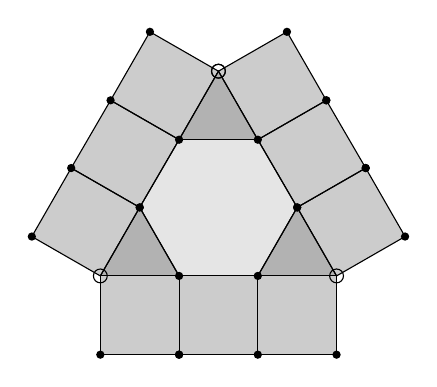
\begin{tikzpicture}[line cap=round,line join=round,>=triangle 45,x=1.0cm,y=1.0cm]
\fill[fill=black,fill opacity=0.1] (2,1) -- (3,1) -- (3.5,1.87) -- (3,2.73) -- (2,2.73) -- (1.5,1.87) -- cycle;
\fill[fill=black,fill opacity=0.2] (1.5,1.87) -- (2,2.73) -- (1.13,3.23) -- (0.63,2.37) -- cycle;
\fill[fill=black,fill opacity=0.2] (1.13,3.23) -- (2,2.73) -- (2.5,3.6) -- (1.63,4.1) -- cycle;
\fill[fill=black,fill opacity=0.2] (1.5,1.87) -- (0.63,2.37) -- (0.13,1.5) -- (1,1) -- cycle;
\fill[fill=black,fill opacity=0.2] (2,1) -- (1,1) -- (1,0) -- (2,0) -- cycle;
\fill[fill=black,fill opacity=0.2] (3,1) -- (2,1) -- (2,0) -- (3,0) -- cycle;
\fill[fill=black,fill opacity=0.2] (3,1) -- (3,0) -- (4,0) -- (4,1) -- cycle;
\fill[fill=black,fill opacity=0.2] (3,2.73) -- (3.5,1.87) -- (4.37,2.37) -- (3.87,3.23) -- cycle;
\fill[fill=black,fill opacity=0.2] (2.5,3.6) -- (3,2.73) -- (3.87,3.23) -- (3.37,4.1) -- cycle;
\fill[fill=black,fill opacity=0.2] (3.5,1.87) -- (4,1) -- (4.87,1.5) -- (4.37,2.37) -- cycle;
\fill[fill=black,fill opacity=0.3] (1,1) -- (2,1) -- (1.5,1.87) -- cycle;
\fill[fill=black,fill opacity=0.3] (3,1) -- (4,1) -- (3.5,1.87) -- cycle;
\fill[fill=black,fill opacity=0.3] (2,2.73) -- (3,2.73) -- (2.5,3.6) -- cycle;
\draw (2,1)-- (3,1);
\draw (3,1)-- (3.5,1.87);
\draw (3.5,1.87)-- (3,2.73);
\draw (3,2.73)-- (2,2.73);
\draw (2,2.73)-- (1.5,1.87);
\draw (1.5,1.87)-- (2,1);
\draw (1.5,1.87)-- (2,2.73);
\draw (2,2.73)-- (1.13,3.23);
\draw (1.13,3.23)-- (0.63,2.37);
\draw (0.63,2.37)-- (1.5,1.87);
\draw (1.13,3.23)-- (2,2.73);
\draw (2,2.73)-- (2.5,3.6);
\draw (2.5,3.6)-- (1.63,4.1);
\draw (1.63,4.1)-- (1.13,3.23);
\draw (1.5,1.87)-- (0.63,2.37);
\draw (0.63,2.37)-- (0.13,1.5);
\draw (0.13,1.5)-- (1,1);
\draw (1,1)-- (1.5,1.87);
\draw (2,1)-- (1,1);
\draw (1,1)-- (1,0);
\draw (1,0)-- (2,0);
\draw (2,0)-- (2,1);
\draw (3,1)-- (2,1);
\draw (2,1)-- (2,0);
\draw (2,0)-- (3,0);
\draw (3,0)-- (3,1);
\draw (3,1)-- (3,0);
\draw (3,0)-- (4,0);
\draw (4,0)-- (4,1);
\draw (4,1)-- (3,1);
\draw (3,2.73)-- (3.5,1.87);
\draw (3.5,1.87)-- (4.37,2.37);
\draw (4.37,2.37)-- (3.87,3.23);
\draw (3.87,3.23)-- (3,2.73);
\draw (2.5,3.6)-- (3,2.73);
\draw (3,2.73)-- (3.87,3.23);
\draw (3.87,3.23)-- (3.37,4.1);
\draw (3.37,4.1)-- (2.5,3.6);
\draw (3.5,1.87)-- (4,1);
\draw (4,1)-- (4.87,1.5);
\draw (4.87,1.5)-- (4.37,2.37);
\draw (4.37,2.37)-- (3.5,1.87);
\draw (1,1)-- (2,1);
\draw (2,1)-- (1.5,1.87);
\draw (1.5,1.87)-- (1,1);
\draw (3,1)-- (4,1);
\draw (4,1)-- (3.5,1.87);
\draw (3.5,1.87)-- (3,1);
\draw (2,2.73)-- (3,2.73);
\draw (3,2.73)-- (2.5,3.6);
\draw (2.5,3.6)-- (2,2.73);
\begin{scriptsize}
\fill [color=black] (2,1) circle (1.5pt);
\fill [color=black] (3,1) circle (1.5pt);
\fill [color=black] (3.5,1.87) circle (1.5pt);
\fill [color=black] (3,2.73) circle (1.5pt);
\fill [color=black] (2,2.73) circle (1.5pt);
\fill [color=black] (1.5,1.87) circle (1.5pt);
\fill [color=black] (1.13,3.23) circle (1.5pt);
\fill [color=black] (0.63,2.37) circle (1.5pt);
\draw [color=black] (2.5,3.6) circle (2.5pt);
\fill [color=black] (1.63,4.1) circle (1.5pt);
\fill [color=black] (0.13,1.5) circle (1.5pt);
\draw [color=black] (1,1) circle (2.5pt);
\fill [color=black] (1,0) circle (1.5pt);
\fill [color=black] (2,0) circle (1.5pt);
\fill [color=black] (2,0) circle (1.5pt);
\fill [color=black] (3,0) circle (1.5pt);
\fill [color=black] (4,0) circle (1.5pt);
\draw [color=black] (4,1) circle (2.5pt);
\fill [color=black] (4.37,2.37) circle (1.5pt);
\fill [color=black] (3.87,3.23) circle (1.5pt);
\fill [color=black] (3.87,3.23) circle (1.5pt);
\fill [color=black] (3.37,4.1) circle (1.5pt);
\fill [color=black] (4.87,1.5) circle (1.5pt);
\fill [color=black] (4.37,2.37) circle (1.5pt);
\fill [color=black] (1.5,1.87) circle (1.5pt);
\fill [color=black] (3.5,1.87) circle (1.5pt);
\draw [color=black] (2.5,3.6) circle (2.5pt);
\end{scriptsize}
\end{tikzpicture}
\end{center}
Összegezve az eredményeket, egyedül a $(4,3,4,6)$ típusú
lefödés ad szabályos lefödést.

Áttérünk a b) alpont megoldására. A következő
ábrán látható lefödés szabályos, ha
tizenkétszögekben, négyzetekben  és hatszö\-gek\-ben
gondolkodunk (minden csúcs $(4,6,12)$ típusú).
\begin{center}
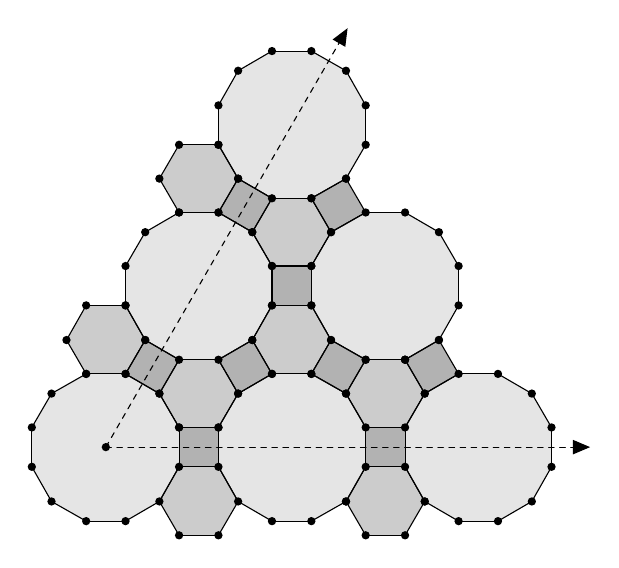
\begin{tikzpicture}[line cap=round,line join=round,>=triangle 45,x=1.0cm,y=1.0cm]
\fill[fill=black,fill opacity=0.2] (1.5,0) -- (2,0) -- (2.25,0.43) -- (2,0.87) -- (1.5,0.87) -- (1.25,0.43) -- cycle;
\fill[fill=black,fill opacity=0.1] (1.25,0.43) -- (1.5,0.87) -- (1.5,1.37) -- (1.25,1.8) -- (0.82,2.05) -- (0.32,2.05) -- (-0.12,1.8) -- (-0.37,1.37) -- (-0.37,0.87) -- (-0.12,0.43) -- (0.32,0.18) -- (0.82,0.18) -- cycle;
\fill[fill=black,fill opacity=0.1] (2,0.87) -- (2.25,0.43) -- (2.68,0.18) -- (3.18,0.18) -- (3.62,0.43) -- (3.87,0.87) -- (3.87,1.37) -- (3.62,1.8) -- (3.18,2.05) -- (2.68,2.05) -- (2.25,1.8) -- (2,1.37) -- cycle;
\fill[fill=black,fill opacity=0.3] (1.5,0.87) -- (2,0.87) -- (2,1.37) -- (1.5,1.37) -- cycle;
\fill[fill=black,fill opacity=0.2] (1.5,1.37) -- (2,1.37) -- (2.25,1.8) -- (2,2.23) -- (1.5,2.23) -- (1.25,1.8) -- cycle;
\fill[fill=black,fill opacity=0.1] (1.5,2.23) -- (2,2.23) -- (2.43,2.48) -- (2.68,2.92) -- (2.68,3.42) -- (2.43,3.85) -- (2,4.1) -- (1.5,4.1) -- (1.07,3.85) -- (0.82,3.42) -- (0.82,2.92) -- (1.07,2.48) -- cycle;
\fill[fill=black,fill opacity=0.3] (2,2.23) -- (2.25,1.8) -- (2.68,2.05) -- (2.43,2.48) -- cycle;
\fill[fill=black,fill opacity=0.3] (1.25,1.8) -- (1.5,2.23) -- (1.07,2.48) -- (0.82,2.05) -- cycle;
\fill[fill=black,fill opacity=0.2] (0.82,2.05) -- (1.07,2.48) -- (0.82,2.92) -- (0.32,2.92) -- (0.07,2.48) -- (0.32,2.05) -- cycle;
\fill[fill=black,fill opacity=0.2] (2.43,2.48) -- (2.68,2.05) -- (3.18,2.05) -- (3.43,2.48) -- (3.18,2.92) -- (2.68,2.92) -- cycle;
\fill[fill=black,fill opacity=0.3] (3.18,2.05) -- (3.62,1.8) -- (3.87,2.23) -- (3.43,2.48) -- cycle;
\fill[fill=black,fill opacity=0.3] (3.87,1.37) -- (3.87,0.87) -- (4.37,0.87) -- (4.37,1.37) -- cycle;
\fill[fill=black,fill opacity=0.1] (4.37,1.37) -- (4.37,0.87) -- (4.62,0.43) -- (5.05,0.18) -- (5.55,0.18) -- (5.98,0.43) -- (6.23,0.87) -- (6.23,1.37) -- (5.98,1.8) -- (5.55,2.05) -- (5.05,2.05) -- (4.62,1.8) -- cycle;
\fill[fill=black,fill opacity=0.1] (3.43,2.48) -- (3.87,2.23) -- (4.37,2.23) -- (4.8,2.48) -- (5.05,2.92) -- (5.05,3.42) -- (4.8,3.85) -- (4.37,4.1) -- (3.87,4.1) -- (3.43,3.85) -- (3.18,3.42) -- (3.18,2.92) -- cycle;
\fill[fill=black,fill opacity=0.2] (4.37,0.87) -- (3.87,0.87) -- (3.62,0.43) -- (3.87,0) -- (4.37,0) -- (4.62,0.43) -- cycle;
\fill[fill=black,fill opacity=0.2] (3.87,1.37) -- (4.37,1.37) -- (4.62,1.8) -- (4.37,2.23) -- (3.87,2.23) -- (3.62,1.8) -- cycle;
\fill[fill=black,fill opacity=0.3] (2.68,2.92) -- (3.18,2.92) -- (3.18,3.42) -- (2.68,3.42) -- cycle;
\fill[fill=black,fill opacity=0.2] (2.68,3.42) -- (3.18,3.42) -- (3.43,3.85) -- (3.18,4.28) -- (2.68,4.28) -- (2.43,3.85) -- cycle;
\fill[fill=black,fill opacity=0.3] (2.43,3.85) -- (2.68,4.28) -- (2.25,4.53) -- (2,4.1) -- cycle;
\fill[fill=black,fill opacity=0.1] (2.68,4.28) -- (3.18,4.28) -- (3.62,4.53) -- (3.87,4.96) -- (3.87,5.46) -- (3.62,5.9) -- (3.18,6.15) -- (2.68,6.15) -- (2.25,5.9) -- (2,5.46) -- (2,4.96) -- (2.25,4.53) -- cycle;
\fill[fill=black,fill opacity=0.3] (3.43,3.85) -- (3.87,4.1) -- (3.62,4.53) -- (3.18,4.28) -- cycle;
\fill[fill=black,fill opacity=0.3] (4.62,1.8) -- (5.05,2.05) -- (4.8,2.48) -- (4.37,2.23) -- cycle;
\fill[fill=black,fill opacity=0.2] (2,4.1) -- (2.25,4.53) -- (2,4.96) -- (1.5,4.96) -- (1.25,4.53) -- (1.5,4.1) -- cycle;
\draw (1.5,0)-- (2,0);
\draw (2,0)-- (2.25,0.43);
\draw (2.25,0.43)-- (2,0.87);
\draw (2,0.87)-- (1.5,0.87);
\draw (1.5,0.87)-- (1.25,0.43);
\draw (1.25,0.43)-- (1.5,0);
\draw (1.25,0.43)-- (1.5,0.87);
\draw (1.5,0.87)-- (1.5,1.37);
\draw (1.5,1.37)-- (1.25,1.8);
\draw (1.25,1.8)-- (0.82,2.05);
\draw (0.82,2.05)-- (0.32,2.05);
\draw (0.32,2.05)-- (-0.12,1.8);
\draw (-0.12,1.8)-- (-0.37,1.37);
\draw (-0.37,1.37)-- (-0.37,0.87);
\draw (-0.37,0.87)-- (-0.12,0.43);
\draw (-0.12,0.43)-- (0.32,0.18);
\draw (0.32,0.18)-- (0.82,0.18);
\draw (0.82,0.18)-- (1.25,0.43);
\draw (2,0.87)-- (2.25,0.43);
\draw (2.25,0.43)-- (2.68,0.18);
\draw (2.68,0.18)-- (3.18,0.18);
\draw (3.18,0.18)-- (3.62,0.43);
\draw (3.62,0.43)-- (3.87,0.87);
\draw (3.87,0.87)-- (3.87,1.37);
\draw (3.87,1.37)-- (3.62,1.8);
\draw (3.62,1.8)-- (3.18,2.05);
\draw (3.18,2.05)-- (2.68,2.05);
\draw (2.68,2.05)-- (2.25,1.8);
\draw (2.25,1.8)-- (2,1.37);
\draw (2,1.37)-- (2,0.87);
\draw (1.5,0.87)-- (2,0.87);
\draw (2,0.87)-- (2,1.37);
\draw (2,1.37)-- (1.5,1.37);
\draw (1.5,1.37)-- (1.5,0.87);
\draw (1.5,1.37)-- (2,1.37);
\draw (2,1.37)-- (2.25,1.8);
\draw (2.25,1.8)-- (2,2.23);
\draw (2,2.23)-- (1.5,2.23);
\draw (1.5,2.23)-- (1.25,1.8);
\draw (1.25,1.8)-- (1.5,1.37);
\draw (1.5,2.23)-- (2,2.23);
\draw (2,2.23)-- (2.43,2.48);
\draw (2.43,2.48)-- (2.68,2.92);
\draw (2.68,2.92)-- (2.68,3.42);
\draw (2.68,3.42)-- (2.43,3.85);
\draw (2.43,3.85)-- (2,4.1);
\draw (2,4.1)-- (1.5,4.1);
\draw (1.5,4.1)-- (1.07,3.85);
\draw (1.07,3.85)-- (0.82,3.42);
\draw (0.82,3.42)-- (0.82,2.92);
\draw (0.82,2.92)-- (1.07,2.48);
\draw (1.07,2.48)-- (1.5,2.23);
\draw (2,2.23)-- (2.25,1.8);
\draw (2.25,1.8)-- (2.68,2.05);
\draw (2.68,2.05)-- (2.43,2.48);
\draw (2.43,2.48)-- (2,2.23);
\draw (1.25,1.8)-- (1.5,2.23);
\draw (1.5,2.23)-- (1.07,2.48);
\draw (1.07,2.48)-- (0.82,2.05);
\draw (0.82,2.05)-- (1.25,1.8);
\draw (0.82,2.05)-- (1.07,2.48);
\draw (1.07,2.48)-- (0.82,2.92);
\draw (0.82,2.92)-- (0.32,2.92);
\draw (0.32,2.92)-- (0.07,2.48);
\draw (0.07,2.48)-- (0.32,2.05);
\draw (0.32,2.05)-- (0.82,2.05);
\draw (2.43,2.48)-- (2.68,2.05);
\draw (2.68,2.05)-- (3.18,2.05);
\draw (3.18,2.05)-- (3.43,2.48);
\draw (3.43,2.48)-- (3.18,2.92);
\draw (3.18,2.92)-- (2.68,2.92);
\draw (2.68,2.92)-- (2.43,2.48);
\draw (3.18,2.05)-- (3.62,1.8);
\draw (3.62,1.8)-- (3.87,2.23);
\draw (3.87,2.23)-- (3.43,2.48);
\draw (3.43,2.48)-- (3.18,2.05);
\draw (3.87,1.37)-- (3.87,0.87);
\draw (3.87,0.87)-- (4.37,0.87);
\draw (4.37,0.87)-- (4.37,1.37);
\draw (4.37,1.37)-- (3.87,1.37);
\draw (4.37,1.37)-- (4.37,0.87);
\draw (4.37,0.87)-- (4.62,0.43);
\draw (4.62,0.43)-- (5.05,0.18);
\draw (5.05,0.18)-- (5.55,0.18);
\draw (5.55,0.18)-- (5.98,0.43);
\draw (5.98,0.43)-- (6.23,0.87);
\draw (6.23,0.87)-- (6.23,1.37);
\draw (6.23,1.37)-- (5.98,1.8);
\draw (5.98,1.8)-- (5.55,2.05);
\draw (5.55,2.05)-- (5.05,2.05);
\draw (5.05,2.05)-- (4.62,1.8);
\draw (4.62,1.8)-- (4.37,1.37);
\draw (3.43,2.48)-- (3.87,2.23);
\draw (3.87,2.23)-- (4.37,2.23);
\draw (4.37,2.23)-- (4.8,2.48);
\draw (4.8,2.48)-- (5.05,2.92);
\draw (5.05,2.92)-- (5.05,3.42);
\draw (5.05,3.42)-- (4.8,3.85);
\draw (4.8,3.85)-- (4.37,4.1);
\draw (4.37,4.1)-- (3.87,4.1);
\draw (3.87,4.1)-- (3.43,3.85);
\draw (3.43,3.85)-- (3.18,3.42);
\draw (3.18,3.42)-- (3.18,2.92);
\draw (3.18,2.92)-- (3.43,2.48);
\draw (4.37,0.87)-- (3.87,0.87);
\draw (3.87,0.87)-- (3.62,0.43);
\draw (3.62,0.43)-- (3.87,0);
\draw (3.87,0)-- (4.37,0);
\draw (4.37,0)-- (4.62,0.43);
\draw (4.62,0.43)-- (4.37,0.87);
\draw (3.87,1.37)-- (4.37,1.37);
\draw (4.37,1.37)-- (4.62,1.8);
\draw (4.62,1.8)-- (4.37,2.23);
\draw (4.37,2.23)-- (3.87,2.23);
\draw (3.87,2.23)-- (3.62,1.8);
\draw (3.62,1.8)-- (3.87,1.37);
\draw (2.68,2.92)-- (3.18,2.92);
\draw (3.18,2.92)-- (3.18,3.42);
\draw (3.18,3.42)-- (2.68,3.42);
\draw (2.68,3.42)-- (2.68,2.92);
\draw (2.68,3.42)-- (3.18,3.42);
\draw (3.18,3.42)-- (3.43,3.85);
\draw (3.43,3.85)-- (3.18,4.28);
\draw (3.18,4.28)-- (2.68,4.28);
\draw (2.68,4.28)-- (2.43,3.85);
\draw (2.43,3.85)-- (2.68,3.42);
\draw (2.43,3.85)-- (2.68,4.28);
\draw (2.68,4.28)-- (2.25,4.53);
\draw (2.25,4.53)-- (2,4.1);
\draw (2,4.1)-- (2.43,3.85);
\draw (2.68,4.28)-- (3.18,4.28);
\draw (3.18,4.28)-- (3.62,4.53);
\draw (3.62,4.53)-- (3.87,4.96);
\draw (3.87,4.96)-- (3.87,5.46);
\draw (3.87,5.46)-- (3.62,5.9);
\draw (3.62,5.9)-- (3.18,6.15);
\draw (3.18,6.15)-- (2.68,6.15);
\draw (2.68,6.15)-- (2.25,5.9);
\draw (2.25,5.9)-- (2,5.46);
\draw (2,5.46)-- (2,4.96);
\draw (2,4.96)-- (2.25,4.53);
\draw (2.25,4.53)-- (2.68,4.28);
\draw (3.43,3.85)-- (3.87,4.1);
\draw (3.87,4.1)-- (3.62,4.53);
\draw (3.62,4.53)-- (3.18,4.28);
\draw (3.18,4.28)-- (3.43,3.85);
\draw (4.62,1.8)-- (5.05,2.05);
\draw (5.05,2.05)-- (4.8,2.48);
\draw (4.8,2.48)-- (4.37,2.23);
\draw (4.37,2.23)-- (4.62,1.8);
\draw [->,dash pattern=on 2pt off 2pt] (0.57,1.12) -- (3.64,6.44);
\draw [->,dash pattern=on 2pt off 2pt] (0.57,1.12) -- (6.72,1.12);
\draw (2,4.1)-- (2.25,4.53);
\draw (2.25,4.53)-- (2,4.96);
\draw (2,4.96)-- (1.5,4.96);
\draw (1.5,4.96)-- (1.25,4.53);
\draw (1.25,4.53)-- (1.5,4.1);
\draw (1.5,4.1)-- (2,4.1);
\begin{scriptsize}
\fill [color=black] (1.5,0) circle (1.5pt);
\fill [color=black] (2,0) circle (1.5pt);
\fill [color=black] (2.25,0.43) circle (1.5pt);
\fill [color=black] (2,0.87) circle (1.5pt);
\fill [color=black] (1.5,0.87) circle (1.5pt);
\fill [color=black] (1.25,0.43) circle (1.5pt);
\fill [color=black] (1.5,1.37) circle (1.5pt);
\fill [color=black] (1.25,1.8) circle (1.5pt);
\fill [color=black] (0.82,2.05) circle (1.5pt);
\fill [color=black] (0.32,2.05) circle (1.5pt);
\fill [color=black] (-0.12,1.8) circle (1.5pt);
\fill [color=black] (-0.37,1.37) circle (1.5pt);
\fill [color=black] (-0.37,0.87) circle (1.5pt);
\fill [color=black] (-0.12,0.43) circle (1.5pt);
\fill [color=black] (0.32,0.18) circle (1.5pt);
\fill [color=black] (0.82,0.18) circle (1.5pt);
\fill [color=black] (2.68,0.18) circle (1.5pt);
\fill [color=black] (3.18,0.18) circle (1.5pt);
\fill [color=black] (3.62,0.43) circle (1.5pt);
\fill [color=black] (3.87,0.87) circle (1.5pt);
\fill [color=black] (3.87,1.37) circle (1.5pt);
\fill [color=black] (3.62,1.8) circle (1.5pt);
\fill [color=black] (3.18,2.05) circle (1.5pt);
\fill [color=black] (2.68,2.05) circle (1.5pt);
\fill [color=black] (2.25,1.8) circle (1.5pt);
\fill [color=black] (2,1.37) circle (1.5pt);
\fill [color=black] (2,1.37) circle (1.5pt);
\fill [color=black] (1.5,1.37) circle (1.5pt);
\fill [color=black] (2.25,1.8) circle (1.5pt);
\fill [color=black] (2,2.23) circle (1.5pt);
\fill [color=black] (1.5,2.23) circle (1.5pt);
\fill [color=black] (1.25,1.8) circle (1.5pt);
\fill [color=black] (2.43,2.48) circle (1.5pt);
\fill [color=black] (2.68,2.92) circle (1.5pt);
\fill [color=black] (2.68,3.42) circle (1.5pt);
\fill [color=black] (2.43,3.85) circle (1.5pt);
\fill [color=black] (2,4.1) circle (1.5pt);
\fill [color=black] (1.5,4.1) circle (1.5pt);
\fill [color=black] (1.07,3.85) circle (1.5pt);
\fill [color=black] (0.82,3.42) circle (1.5pt);
\fill [color=black] (0.82,2.92) circle (1.5pt);
\fill [color=black] (1.07,2.48) circle (1.5pt);
\fill [color=black] (2.68,2.05) circle (1.5pt);
\fill [color=black] (2.43,2.48) circle (1.5pt);
\fill [color=black] (1.07,2.48) circle (1.5pt);
\fill [color=black] (0.82,2.05) circle (1.5pt);
\fill [color=black] (0.82,2.92) circle (1.5pt);
\fill [color=black] (0.32,2.92) circle (1.5pt);
\fill [color=black] (0.07,2.48) circle (1.5pt);
\fill [color=black] (0.32,2.05) circle (1.5pt);
\fill [color=black] (3.18,2.05) circle (1.5pt);
\fill [color=black] (3.43,2.48) circle (1.5pt);
\fill [color=black] (3.18,2.92) circle (1.5pt);
\fill [color=black] (2.68,2.92) circle (1.5pt);
\fill [color=black] (0.57,1.12) circle (1.5pt);
\fill [color=black] (3.87,2.23) circle (1.5pt);
\fill [color=black] (3.43,2.48) circle (1.5pt);
\fill [color=black] (4.37,0.87) circle (1.5pt);
\fill [color=black] (4.37,1.37) circle (1.5pt);
\fill [color=black] (4.62,0.43) circle (1.5pt);
\fill [color=black] (5.05,0.18) circle (1.5pt);
\fill [color=black] (5.55,0.18) circle (1.5pt);
\fill [color=black] (5.98,0.43) circle (1.5pt);
\fill [color=black] (6.23,0.87) circle (1.5pt);
\fill [color=black] (6.23,1.37) circle (1.5pt);
\fill [color=black] (5.98,1.8) circle (1.5pt);
\fill [color=black] (5.55,2.05) circle (1.5pt);
\fill [color=black] (5.05,2.05) circle (1.5pt);
\fill [color=black] (4.62,1.8) circle (1.5pt);
\fill [color=black] (4.37,2.23) circle (1.5pt);
\fill [color=black] (4.8,2.48) circle (1.5pt);
\fill [color=black] (5.05,2.92) circle (1.5pt);
\fill [color=black] (5.05,3.42) circle (1.5pt);
\fill [color=black] (4.8,3.85) circle (1.5pt);
\fill [color=black] (4.37,4.1) circle (1.5pt);
\fill [color=black] (3.87,4.1) circle (1.5pt);
\fill [color=black] (3.43,3.85) circle (1.5pt);
\fill [color=black] (3.18,3.42) circle (1.5pt);
\fill [color=black] (3.18,2.92) circle (1.5pt);
\fill [color=black] (3.62,0.43) circle (1.5pt);
\fill [color=black] (3.87,0) circle (1.5pt);
\fill [color=black] (4.37,0) circle (1.5pt);
\fill [color=black] (4.62,0.43) circle (1.5pt);
\fill [color=black] (4.62,1.8) circle (1.5pt);
\fill [color=black] (4.37,2.23) circle (1.5pt);
\fill [color=black] (3.87,2.23) circle (1.5pt);
\fill [color=black] (3.62,1.8) circle (1.5pt);
\fill [color=black] (3.18,3.42) circle (1.5pt);
\fill [color=black] (2.68,3.42) circle (1.5pt);
\fill [color=black] (3.43,3.85) circle (1.5pt);
\fill [color=black] (3.18,4.28) circle (1.5pt);
\fill [color=black] (2.68,4.28) circle (1.5pt);
\fill [color=black] (2.43,3.85) circle (1.5pt);
\fill [color=black] (2.25,4.53) circle (1.5pt);
\fill [color=black] (2,4.1) circle (1.5pt);
\fill [color=black] (3.62,4.53) circle (1.5pt);
\fill [color=black] (3.87,4.96) circle (1.5pt);
\fill [color=black] (3.87,5.46) circle (1.5pt);
\fill [color=black] (3.62,5.9) circle (1.5pt);
\fill [color=black] (3.18,6.15) circle (1.5pt);
\fill [color=black] (2.68,6.15) circle (1.5pt);
\fill [color=black] (2.25,5.9) circle (1.5pt);
\fill [color=black] (2,5.46) circle (1.5pt);
\fill [color=black] (2,4.96) circle (1.5pt);
\fill [color=black] (2.25,4.53) circle (1.5pt);
\fill [color=black] (3.62,4.53) circle (1.5pt);
\fill [color=black] (3.18,4.28) circle (1.5pt);
\fill [color=black] (4.8,2.48) circle (1.5pt);
\fill [color=black] (4.37,2.23) circle (1.5pt);
\fill [color=black] (2,4.96) circle (1.5pt);
\fill [color=black] (1.5,4.96) circle (1.5pt);
\fill [color=black] (1.25,4.53) circle (1.5pt);
\fill [color=black] (1.5,4.1) circle (1.5pt);
\end{scriptsize}
\end{tikzpicture}
\end{center}
Viszont minden tizenkétszöget az a) alpont alapján
egyértelműen háromszögekre,
 négy\-ze\-te\-kre és hatszögekre bonthatunk. Ez a felbontás lehet olyan, hogy egy tizenkétszög
 belsejében elhelyezkedő négyzet egy kinti négyzettel csak csúcsban, vagy élben is
 érint\-kezzen. Ezt minden tizenkétszög esetén tetszőlegesen megvá\-laszt\-hat\-juk, és ezért
 végtelen sok kért lefödést kapunk. Valóban, induljunk ki az egyetlen szabályos
 lefödésből és azonosítsunk be egy tizenkétszöget. Ezután, kúp alakban az ábra
 szerint haladva azonosítsunk be további tizenkétszögeket az előző ábra szerint
 (egy speciális ,,háromszögrácsot'' kapunk, amelynek csúcsai a tizenkétszögek, és az
 őket összekötő alakzatok a négyzetek). Mind\-egyik kiválasztott tizenkétszög kétféle színezést határoz meg, de végtelen sok tizenkétszöget választottunk.


\end{document}